\import{./}{tokens-grammar.tex}

\subsection{Takeaways}

\begin{enumerate}
    \item Operator precedence is directly encoded into the grammar in 6 different precedence levels.
    \item Both boolean and arithmetic operators share the same expressions. The interpreter will automatically cast the right hand side of an expression to the correct type if possible.
    \item The grammar supports JSON literals as well as simple JSONPath accessors in both assignment and retrieval.
\end{enumerate}

\section{Semantics}

\subsection{Statements}

Statements can be one of the following:

\begin{center}
    \begin{enumerate}
        \item An assignment. Only one assignment operator is supported: `='.
        \item A function call.
        \item A HTTP method call.
        \item The break keyword.
        \item Test an expression for a truthy value. This will be talked about more in the `Test Suite' section.
        \item A `while' loop. The condition of which is an expression. This is explained more in the \hyperref[sec:expressions]{`Expressions'} subsection.
        \item A `for' loop. Supports either the ``traditional" C-style format or the iterator style format. The iterator style `for' loop has an optional additional iterator assignment for key-value pair iteration or index-value iteration.
        \item The batch statement which will execute HTTP method calls nested within it in parallel.
        \item A function definition.
        \item An `if-elif-else' block.
        \item A `NOP'. Defined by a statement followed by a singular semi-colon.
    \end{enumerate}
\end{center}

\subsection{Variables and values}

The possible value types are strings, floats, integers, arrays, objects, `true'/`false' and `null'. This matches the types available in JSON. In fact the type of each value will be determined by using the Golang JSON parser on the string representation of the value. Some other semantics:

\begin{center}
    \begin{itemize}
        \item Variables can be modified using `JSON path'.
        \item Variable assignment will carry out a \textbf{deep copy}.
        \item \textbf{Variables are always passed by reference} and expressions are passed by value.
        \item \textbf{Variables are declared and defined} when a new \textbf{root identifier} is used in a JSONPath assignment that \textbf{doesn't exist} in the \textbf{current scope}.
        \item \textbf{Variables are set} when the root identifier \textbf{exists} in the \textbf{current scope}.
        \item \textbf{Variables are filled sparsely} when a \textbf{JSONPath accessing a non-existent sublevel} of the JSON is assigned to. For instance:
        \begin{verbatim}
            hello_world = {
                "hello": "world"
            };
            hello_world.world[1].hello = "world";
            /*
            hello_world = {
                "hello": "world",
                "world": [
                    null,
                    {"hello": "world"}
                ]
            }
            */
        \end{verbatim}
        \item As mentioned earlier, right hand values of operations are cast to the appropriate type if they can be. 
    \end{itemize}
\end{center}

\subsection{JSON path}

The grammar for the language supports rudimentary JSON path expressions. This includes the standard `.' property accessing or the string indexing style. Below are some valid JSON path expressions:

\begin{figure}[H]
    \begin{center}
        \begin{verbatim}
            json[0].path.is.cool
            json[0]["path"].is.["cool"]
            json[x + 2]["path"].is.["co" + "ol"]
        \end{verbatim}
    \end{center}
    \vspace{-1.5em}
    \cprotect\caption{Examples of some valid JSON paths. These all access the \verb|json| variable.}
\end{figure}

When accessing a variable using JSONPath, the variable that is being accessed is called the \textbf{root identifier/property}. This is the first identifier in the JSONPath.

\begin{verbatim}
    // Here the variable that is being accessed
    // is the "json" variable.
    json.hello.world
\end{verbatim}

A JSONPath is constructed from \textbf{properties} and \textbf{parts}. A property is an identifier which directly correlates to a key within an object. A part is an expression surrounded by square braces.

Each part's expression is first evaluated. If the result of this expression is a value of type String then the part will be treated as a property. If the value of the result is of type Number, then the value will be treated as an access to an array. If the value is not of type String or Number, then the interpreter will first try to cast the value to a Number, and then to a String. If the value cannot be cast to either, an error is returned.

\subsubsection{Getting}
\label{sec:jsonpath-getting}

A JSONPath that is used to `get' a value, will not produce an error if the JSONPath doesn't point to a value. Instead the JSONPath will return a `null' value.

Parts that evaluate to Numbers can also be negative if \verb|abs(i) - 1| is less than the length of the Array to access. Negative numbers allow access from the tail of the Array. For instance:

\begin{verbatim}
    a = [1, 2, 3];
    $print(a[-1], a[-2], a[-3]);
    // Output: 3 2 1
\end{verbatim}

\subsubsection{Setting}
\label{sec:jsonpath-setting}

JSON paths can be assigned to. This sets the appropriate property of the variable. This is done recursively by reconstructing the entire value from the bottom-up. Each recursive call takes the current value, the value to set to, as well as the path remaining to evaluate (an array of properties and parts).

\begin{center}
    For each property/part in the JSONPath, the following considerations are made.
    \begin{itemize}
        \item If we have no path remaining, then we will return the value we are setting to.
        \item If the current value is `null' then we won't pop the next property/path from the JSONPath. Instead, we will create a new Object, if the current path evaluates to a String, or a new Array, if the current path evaluates to a Number.
        \item For each of the following actions we will first pop the next item from the remaining path...
        \begin{itemize}
            \item If the current value is an \textbf{Object}...
            \begin{itemize}
                \item \textbf{If the current path item is not a filter expression...}
                \begin{itemize}
                    \item \textbf{If the current path item is a String}, then we will treat it as a key of the Object. We will set the value of the key in the current Object to be the output of a recursive call of the setter function. The current value to pass into the recursive call depends on whether the key already exists in the Object. If it does then we will pass in the value of the key. If it doesn't then we will pass in `null'.
                    \item \textbf{If the current path item is a Number}, then we will order the keys within the Object lexicographically and set the \verb|i|-th key's value using the technique described above. Where \verb|i| is the current path item.
                \end{itemize}
                \item \textbf{Otherwise}, each key-value pair within the Object will be iterated over. At the beginning of each iteration, \verb|curr| will be set to an Object (\verb|{"key": ..., "value": ...}|) containing the key and the value of the currently iterated node. The Block defined within the filter will then be executed, with the value returned by this Block, being cast to a Boolean. If \verb|true|, the currently iterated node will be recursed down using the node's value.
            \end{itemize}
            \item If the current value is an \textbf{Array}...
            \begin{itemize}
                \item \textbf{If the current path item is a Number}, then we will first check if a negative index lookup can be performed as described in the `\hyperref[sec:jsonpath-getting]{Getting}' section...
                \begin{itemize}
                    \item If so, then we will set the index of the Array to be the output of the recursive call to the setter function called with the element currently at that index.
                    \item If not, then we will set each element of the Array up to the index described by the Number to `null' and finally recurse down the index to set, calling the recursive function with `null'.
                \end{itemize}
                \item \textbf{If the current path item is a Filter and not a String}, then we will execute the filter in a very similar way to how it executed on an Object. However, instead we supply the current index of the node as the \verb|key| of the \verb|curr| Object.
            \end{itemize}
            \item If the current value has \textbf{any other type}...
            \begin{itemize}
                \item \textbf{If the current path item is a String}, then we will wrap the current value into an Object with the value residing in a key-value pair of the key \verb|""|. We will then recurse down the key with the value of the current path item, calling the recursive function with `null'. \verb|""| was chosen as the `default key', because it will always be sorted lexicographically as the first key. This means that the value which used to reside there can be accessed by a part such as \verb|[""]| or \verb|[0]|.
                \item \textbf{If the current path item is not a String}...
                \begin{itemize}
                    \item If the current value is a \textbf{String} and the \textbf{current path item is a Filter}, then we will execute the filter in a similar way to Arrays. For every character within the String we recurse down, we will also cast the returned value to a String and append it to a temporary set. We will also mark the current index. After iterating over all the characters in the String, a bulk replacement of all the characters at the marked indices will be replaced by the Strings in the temporary set.
                    \item If the current value is a \textbf{String} and the \textbf{current path item is a Number}, then we will find the correct character within the String. If the Number is negative, we take the absolute of it minus one to get \verb|i|. Otherwise, the Number is \verb|i|. If \verb|i < len(String)| then we will set \verb|i| to \verb|i % len(String)| and get the character at position \verb|i|, otherwise if Number is negative then we will return an error. Otherwise, we will use the default character value: \verb|" "|. We then recurse down this character value. The return of this recursive call is cast to a String. If \verb|i| is greater than or equal to the length of the String, we will insert whitespace up until the \verb|i|-th position, at which point we will write the value that was just cast to a String. If \verb|i| is less than the length of the String, then we set the \verb|i|-th character to be the value that was just cast to a String.
                    \item \textbf{Otherwise}, we will wrap the current value into an Array. If we let the current path value be denoted by \verb|i|, then first we will create an Array with \verb|i + 2| spaces. Inserting the existing value in space \verb|i + 1| and recursing down the \verb|i|-th space, calling the recursive function with `null'.
                \end{itemize}
            \end{itemize}
        \end{itemize}
    \end{itemize}
\end{center}

If the value being set is a Function type then we'll construct a new FunctionDefinition AST node, that will float outside the AST. This node will contain the body and parameters of the Function value that is being set, but will point to the JSONPath AST node of the variable that it is being assigned to.

\subsection{Expressions}
\label{sec:expressions}

Both \textbf{boolean and arithmetic expressions are a part of the same precedence hierarchy}. \textbf{All operators are left-to-right associative}.

\subsubsection{Operator precedence}

\begin{figure}[H]
    \begin{center}
        \begin{tabular}{| m{2cm} | m{2cm} | m{5cm} |}
            \hline
            Precedence & Operators & Description\\
            \hline
            \textbf{0} & \verb|* / %| & Multiplication, division, and modulus\\
            \hline
            \textbf{1} & \verb|+ -| & Addition and subtraction\\
            \hline
            \textbf{2} & \verb|< > <= >=| & Less than, greater than, less than or equal to, and greater than or equal to\\
            \hline
            \textbf{3} & \verb|== !=| & Equal and not equal\\
            \hline
            \textbf{4} & \verb|&&| & Logical and\\
            \hline
            \textbf{5} & \verb+||+ & Logical or\\
            \hline
        \end{tabular}
    \end{center}
    \caption{Operators and their precedence from highest precedence (top) to lowest precedence (bottom)}
\end{figure}

Expressions, and subsequently operators, are evaluated from left to right. Most operator actions involve casting the right-hand side into the type of the value on the left-hand side, then finally performing the operation. This can be used to the benefit of the programmer for various needs, such as casting a value to another type.

\begin{verbatim}
    // Here the Array will be cast to a Number, which will 
    // result in the Array's length
    length = 0 + [1, 2, 3];
\end{verbatim}

\subsubsection{Conditions}

In statements that require conditions (such as `if-elif-else', `while', and `for' statements) a purely arithmetic, a purely logical operator expression, or a mixed expression can all be used. If the expression does not result in a value of a Boolean type, then the result will be cast into a Boolean using the truthy and falsy values below.

\begin{figure}[H]
    \begin{center}
        \begin{tabular}{| c | c | c |}
            \hline
            Type & Truthy value & Falsy value\\
            \hline
            Boolean & \verb|true| & \verb|false|\\
            \hline
            null & & \verb|null|\\
            \hline
            Number & \verb|!= 0| & \verb|0|\\
            \hline
            String & \verb|"..."| & \verb|""|\\
            \hline
            Object & \verb|{...}| & \verb|{}|\\
            \hline
            Array & \verb|[...]| & \verb|[]|\\
            \hline
        \end{tabular}
    \end{center}
    \caption{Table of truthy and falsy values of each type}
\end{figure}

\subsection{Operators}
\label{sec:operatorvaluerel}

Instead of having built-in functions for operations such as appending to an array, removing from an array, merging objects, etc. Operators, perform most of these actions. The following operators remain unchanged for all types:

\begin{itemize}
    \item \textbf{Equal}: \textbf{Deep} equal. \textbf{Returns boolean}.
    \item \textbf{Not-equal}: \textbf{Deep} not-equal. \textbf{Returns boolean}.
    \item \textbf{Less-than, greater-than, less-than or equal, greater-than or equal}: First checks if the first operand is of type Number or String (comparable types). If not then the first operand will be tried to be cast into a Number, and then a String, and if it still cannot, an error will be returned. Then the second operand is cast into the type of the newly cast first operand, returning an error if required. Then these newly cast operands are compared and a Boolean value is returned. \textbf{Null cannot be compared}.
    \item \textbf{Logical And}: Compares by casting both operands to boolean values.
    \item \textbf{Logical Or}: Compares by casting both operands to boolean values.
\end{itemize}

Below, is a run through of each supported operation for each type. \textit{Note that this presumes that all of the types below are on the left-hand side of the operator.}

\subsubsection{Objects}

\begin{itemize}
    \item \textbf{Addition}: Will merge the RHS into the left overriding any values with the same key.
    \item \textbf{Subtraction}: Left value will have key-value pairs found in right value deleted from it.
    \item \textbf{Divide}: Right associative set difference. $op2 - op1$ or $op2 \setminus op1$. This will still have to cast the RHS to an Object.
\end{itemize}

\subsubsection{Arrays}

\begin{itemize}
    \item \textbf{Addition}: If the right-hand value is not an Array, then it will be appended to the left value. If the right-hand value is an Array then the elements of the right-hand Array will be appended to the left-hand Array. Note that the RHS is \textbf{never cast} to the Array type.
    \item \textbf{Subtraction}: Subtract elements from Array. All elements on the LHS Equal to the elements in the RHS will be removed. If the element is null then the head of the Array is removed. The same element cannot be removed more than once in the same operation. This includes `null'.
\end{itemize}

\subsubsection{Strings}

\begin{itemize}
    \item \textbf{Multiply}: Will repeat the String on the left $n$ times, where $n$ is the RHS cast to a Number.
    \item \textbf{Modulus}: If the RHS value is not of type String, then the RHS will be cast to an Array. String interpolation is performed on the String on the LHS using the verb `\verb|%%|'. If the RHS value is a String then this String will be treated as a singleton array, and the String interpolation will be carried out using this value.
    \item \textbf{Addition}: Concatenation.
    \item \textbf{Subtraction}: Depending on the type of the RHS the following will happen:
    \begin{itemize}
        \item \textbf{Number}:  Remove the last n digits from the String.
        \item \textbf{String}:  Remove all occurrences of the RHS from the LHS.
        \item \textbf{Object}:  Replaces all occurrences of RHS's keys with String versions of their values.
        \item \textbf{Array}:   Casts each element in the array to a string and removes all occurrences of each from the LHS.
        \item \textbf{Default}: Casts RHS to string and removes all occurrences of it from the LHS.
    \end{itemize}
\end{itemize}

\subsubsection{Numbers}

All operators work as expected.

\subsubsection{Booleans}

\begin{itemize}
    \item \textbf{Multiply}: Same as Logical And.
    \item \textbf{Divide}: Inverse of Logical And (NAND).
    \item \textbf{Modulus}: The material conditional/Implies that. $op1 \rightarrow op2$.
    \item \textbf{Addition}: Same as Logical Or.
    \item \textbf{Subtraction}: Inverse of Logical Or (NOR).
\end{itemize}

\subsubsection{Nulls}

Multiply, Divide, Modulus, Addition, and Subtraction will all `nullify' the operation (result in `null'). Null cannot be compared but can be used in logical expressions where it will be cast into `false'.

\subsection{Casting}

All casting function are stored within a matrix, with types to cast from represented as rows of this matrix, and types to cast to represented as columns. Casting a value to the type that is the type of the value will always result in the same value.

\begin{center}
\textit{If a type is not mentioned in any of the sections below it means that the type cannot be cast to the missing type, and will return an error.}
\end{center}

\subsubsection{Casting from Objects}

\begin{itemize}
    \item \textbf{To Array}: Extracts the keys from the Object. Will always be an Array of Strings.
    \item \textbf{To String}: Marshals the Object as a JSON string.
    \item \textbf{To Number}: Returns the number of keys in the Object.
    \item \textbf{To Boolean}: If the Object is not empty (length is greater than 0) then the Object is truthy, otherwise the Object is falsy.
\end{itemize}

\subsubsection{Casting from Arrays}

\begin{itemize}
    \item \textbf{To Object}: Creates an Object where each key is an index of an element in the Array, the value of which is the element that lies at that index.
    \item \textbf{To String}: Marshals the Object as a JSON string.
    \item \textbf{To Number}: Returns the number of elements in the Array.
    \item \textbf{To Boolean}: If the Array is not empty then the Array is truthy, otherwise the Array is falsy.
\end{itemize}

\subsubsection{Casting from Strings}

\begin{itemize}
    \item \textbf{To Object}: Attempts to parse the String into a JSON Object.
    \item \textbf{To Array}: Attempts to parse the String into a JSON Array.
    \item \textbf{To Number}: Attempts to parse the String to an integer, then a float, and will finally just take the length of the String.
    \item \textbf{To Boolean}: If the String is not empty then the String is truthy, otherwise the String is falsy.
\end{itemize}

\subsubsection{Casting from Numbers}

\begin{itemize}
    \item \textbf{To Object}: Constructs a singleton Object where the key is the String representation of the Number, and the value is Null.
    \item \textbf{To Array}: Constructs a singleton Array where the first and only element is the Number.
    \item \textbf{To String}: Marshals the Number as a JSON number.
    \item \textbf{To Boolean}: Whether or not the Number is greater than 0.
\end{itemize}

\subsubsection{Casting from Boolean}

\begin{itemize}
    \item \textbf{To Object}: Constructs a singleton Object where the key is the String representation of the Boolean, and the value is Null.
    \item \textbf{To Array}: Constructs a singleton Array where the first and only element is the Boolean.
    \item \textbf{To String}: Marshals the Boolean as a JSON boolean.
    \item \textbf{To Number}: 0 if false, 1 otherwise.
\end{itemize}

\subsubsection{Casting from Null}

\begin{itemize}
    \item \textbf{To Object}: Constructs a singleton Object where the key is the String representation of Null (\verb|null|), and the value is Null.
    \item \textbf{To Array}: Constructs a singleton Array where the first and only element is Null.
    \item \textbf{To String}: \verb|null|.
    \item \textbf{To Number}: Returns false.
\end{itemize}

\subsubsection{Casting from Functions}

\begin{itemize}
    \item \textbf{To String}: \verb|function:JSON_PATH:SAFE_PTR|.
\end{itemize}

\section{Functions}

Functions are defined as follows:

\begin{verbatim}
function foo(a, b)
    return a + b;
end;
\end{verbatim}

This places the value \verb|foo| on the heap of the current \hyperref[sec:function-call-stack]{stack frame}, with a value of type Function. This value points to the FunctionDefinition AST node of the defined function. In sttp this value will be treated as a String in the format: \verb|function:JSON_PATH:SAFE_PTR|.

\subsection{Call Stack}
\label{sec:function-call-stack}

Each time a function is called, the Function value will be fetched using JSONPath. If the value returned by the JSONPath is not a Function type, then the builtin function table will be checked, if the function is still not found then an Uncallable error is thrown.

If the function call is to a user-defined function within the AST. The arguments that were provided to the function are evaluated. Then a new stack frame is allocated and placed on the top of the stack. This stack frame contains a pointer back to the FunctionCall AST node, as well as a pointer to the FunctionDefinition AST node which contains the name, body, and parameters of the function that was called.

If the function call is to a builtin or is a HTTP method call, then no stack frame is allocated. The corresponding Golang code is executed instead. At the beginning of each sttp program an initial stack frame is assigned which points to nil for both FunctionCall and FunctionDefinition pointers.

\subsection{Heap}
\label{sec:function-heap}

Along with these pointers a new heap is assigned. This contains a mapping of variable names to sttp values. All values defined as a global variable from the previous stack frame are copied by reference over to the new stack stack frame. Each argument is assigned to the JSONPath defined in the function's parameters and placed on this heap. If there is no argument for a defined function parameter, then that parameter will be set to `null'. If there are more arguments provided then there are parameters, then a MoreArgsThanParams error is thrown. A `self' value is also placed on the heap which contains the value pointed to by the root property of the JSONPath of the function. For instance:

\begin{verbatim}
hello_world = {"name": "John Smith"};

function hello_world.hello()
    $print("Hello", self.name + "!");
end;

hello_world.hello();
// Output: Hello John Smith!
\end{verbatim}

Parameters are defined in order from left to right, with the `self' parameter defined first. This can give way to some interesting behaviour such as the following:

\begin{verbatim}
foo = {"name": "John Smith"};

// "foo" is populated with new keys "a", "b", and "c"
function foo.zoo(self.a, self.b, foo.c)
    self.result = self.a * self.b * self.c;
end;

foo.zoo(3, 7, 2);
print(foo);
// Output: {
//     "a": 3,
//     "b": 7,
//     "c": 2,
//     "name": "John Smith",
//     "result": 42,
//     "zoo": "function:foo.zoo:XXXXXXX"
// }
\end{verbatim}

Once the function has completed execution, the current stack frame is popped from the callstack and de-allocated by Go.

\section{Error handling}

Each evaluator for each node in the AST is able to return an error and a result. If an error occurs within a leaf node of the AST, then this error will be passed all the way up to the root of the AST, or up until a Try-Catch AST node.

\begin{center}
    The try catch statement works in the following way:
    \begin{verbatim}
        try this
            a = [1, 2, 3];
            // Error occurs on below line
            $print(a[-4]);
        catch as e then
            $print(e);
        end;
    \end{verbatim}
\end{center}

Definition of a variable to store the exception within is mandatory and has to be an identifier, rather than a JSONPath. The value stored within the identifier follows the rules defined below:

\begin{enumerate}
    \item If the error is from a \verb|throw| statement then the value placed into the identifier will match the value of the result of the expression in the \verb|throw| statement. If no expression is given for the \verb|throw| statement, then `null' will be stored in the identifier.
    \item If the error is \textbf{not} from a \verb|throw| statement then the value is constructed in the following way:
    \begin{center}
        \begin{verbatim}
{
    "type":   The name/type of the error (string),
    "error":  The error message (string),
    "subset": The subset which the error is 
                a part of (string)
    // The below two keys will only be added to
    // the value if there is context available
    // from within the package that created the
    // error.
    "pos": {
        // The column number that the error
        // occurred on
        "col": 0.0,
        // The sttp file in which the error
        // occurred in
        "filename": "*.sttp",
        // The line number that the error
        // occurred on
        "line": 0.0,
    },
    // The callstack is converted to an sttp 
    // value. It only converts the most recent
    // couple of stack frames
    "callstack": [
        {
            "parent": {
                "pos": {"line": ..., "col": ..., "filename": ...},
                "function": "FunctionDeclaration pointer",
                "string": "Pretty printed sttp code",
            },
            "caller": {
                "pos": {"line": ..., "col": ..., "filename": ...},
                "string": "Pretty printed sttp code",
            },
        },
        ...
    ]
}
        \end{verbatim}
    \end{center}
\end{enumerate}

\subsection{Error types}

\subsubsection{Subset: Runtime}

Table of errors that occur at runtime.

\begin{center}
    \small
    \begin{tabular}{| m{5cm} | m{5cm} |}
        \hline
        Name & Description\\
        \hline
        StackOverflow & Pushed one too many stack frames onto the call stack. Default max stack size is 500.\\
        \hline
	    StackUnderFlow & Popped one too many stack frames off the call stack.\\
        \hline
	    CannotFindType & Cannot find the type for a value. If the value is not a JSON type.\\
        \hline
	    CannotCast & Cannot cast a value of type $x$ into a value of type $y$.\\
        \hline
	    CannotFindLength & Cannot find the length of a value.\\
        \hline
	    InvalidOperation & Operation $z$ between a value of type $x$ and a value of type $y$ is not defined.\\
        \hline
	    StringManipulationError & Error whilst manipulating a string using all string manipulation operators.\\
        \hline
	    JSONPathError & Cannot access a value with a property/part.\\
        \hline
	    Uncallable & Only values of the Function type can be called. Otherwise, this error is thrown.\\
        \hline
	    MoreArgsThanParams & More arguments were given to a function during a function call than there are defined parameters in the function's definition.\\
        \hline
	    MethodParamNotOptional & A parameter within a HTTP method call is not optional.\\
        \hline
        MethodCallMismatchInBatch & The pointer to a result for a batched method call does not match the currently evaluated method call.\\
        \hline
    \end{tabular}
\end{center}
\normalsize

\subsubsection{Subset: Structure}

\begin{center}
    \small
    \begin{tabular}{| m{5cm} | m{5cm} |}
        \hline
        ImmutableValue & The value being assigned on the heap is read-only. Occurs when trying to set an uncopied Function.\\
        \hline
        BatchWithinBatch & When a batch statement occurs within a batch statement.\\
        \hline
        NoTestSuite & Cannot execute a test statement as the test results array has not yet been initialised.\\
        \hline
        HeapEntryDoesNotExist & Root JSONPath property does not exist within the heap.\\
        \hline
    \end{tabular}
\end{center}
\normalsize

\section{Builtins}
\label{sec:builtins}

Unlike \hyperref[sec:method-calls]{Method Calls}, they share the same AST nodes as Function Calls. However, unlike Function Calls and Method Calls they take an array of \textbf{uncomputed arguments}. This is because some builtins, such as \verb|free|, need context of the AST nodes passed into the builtin call as expressions. Inside the Function Call AST node, if a function cannot be found at the JSONPath of the Function Call, then if the JSONPath only has a root property, the root property will be used to lookup in a map of builtins. If found, the builtin is called and \textbf{no} stack frame is allocated on the call stack.

\cprotect\subsection{\verb|$print(value Any...) -> Null|}

\verb|print| is a simple print function that will print to the stdout file currently being used by the VM. Each \verb|value| given to \verb|print| will be separated by a single space character. Value's will be printed as their minimum (no whitespace, indents or newlines) JSON representations. If the value is a String, then the Go representation of the string will be printed instead (no surrounding double quotes, newlines and other special characters will not be escaped). A single newline character will always be printed at the end, after all values are printed.

\subsubsection{Examples}

\begin{verbatim}
a = { "hello": "\"John\"" };
$print(a);
$print(a.hello);
$print("%% Smith" % a.hello);
$print("hello\nworld!");

// Output:
// {"hello":"\"John\""}
// "John"
// "John" Smith
// hello
// world!
\end{verbatim}

\cprotect\subsection{\verb|$free(path Expression...) -> Null|}

\verb|free| is a special builtin which does not compute the arguments that are passed to it. Instead it analyses the leftmost factor of each Expression passed to it to check if it is a JSONPath AST node. If it is, then the value at that JSONPath will either be `deleted' from the heap if the JSONPath is only a root property, or set to Null if it isn't.

If one of the given Expressions does not contain a JSONPath AST node, then an \verb|InvalidOperation| error will be thrown. Even though sttp is not meant for long running code the usage of \verb|free| is encouraged. This is because sttp does not have a garbage collector of any form.

\subsubsection{Examples}

\begin{verbatim}
a.b.c = "hello";
a.b = a.b + {"foo": "bar"};
a = a + {"baz": "bor"};

$print("a =", a);

$free(a.b.c + 1, a.b.foo * 3.142);

$print("a =", a);

try this
    $free("hello" / "blah" + a);
catch as e then
    $print(e);
end;

b = null;
c = "this is the variable c";

$print("before:");
$print("a =", a);
$print("b =", b);
$print("c =", c);
$print("e =", e);

$free(a, b, c, e);

$print("after:");
$print("a =", a);
$print("b =", b);
$print("c =", c);
$print("e =", e);
// Output:
// a = {"b":{"c":"hello","foo":"bar"},"baz":"bor"}
// a = {"b":{"c":null,"foo":null},"baz":"bor"}
// {"callstack":[],"error":"example_12:12:6: cannot carry out operation \"builtin:delete\" for non-JSONPath value: \"\"hello\"\" and delete","pos":{"col":6,"filename":"example_12","line":12},"subset":"RuntimeError","type":"InvalidOperation"}
// before:
// a = {"b":{"c":null,"foo":null},"baz":"bor"}
// b = null
// c = this is the variable c
// e = {"callstack":[],"error":"example_12:12:6: cannot carry out operation \"builtin:delete\" for non-JSONPath value: \"\"hello\"\" and delete","pos":{"col":6,"filename":"example_12","line":12},"subset":"RuntimeError","type":"InvalidOperation"}
// after:
// a = null
// b = null
// c = null
// e = null
\end{verbatim}

\cprotect\subsection{\verb|$find(searching Any, search_schemas Object...) -> Array|}
\label{sec:builtin-find}

\verb|find| will find the given \verb|search_schema|s within the \verb|searching| value. A search schema will be searched within the value as follows:

\begin{itemize}
    \item Each element and sub-element of the given \verb|searching| value will be searched recursively, depth-first, left to right.
    \item If the current search schema is an Object, then all keys within the search schema \textbf{must} exist within the currently searched element/sub-element.
    \item If the key \verb|""| (empty string) exists within an Object search schema then this counts as a match for any element/sub-element of the currently searched value.
    \item If the currently searched value is an Array and the current search schema is an Object, each index in the searched Array will first be converted to a String and then checked for its existence in the search schema.
    \item If the search schema is a String and the currently searched value is also a String, then if the search schema String is contained within the currently searched value String, then this counts as a match.
    \item Any other combination of search schema type and search value type that is not mentioned above will be handled by performing a deep equal on the search schema and the searched value.
\end{itemize}

This is how all the find builtins work. \verb|find| is unique as it returns the leftmost, deepest value, and nothing else.

\subsubsection{Examples}

\begin{center}
    Example 1
\begin{verbatim}
a = {
    "foo": "bar",
    "baz": {
        "results": [
            {
                "no": 1,
                "type": "string",
                "data": "this is the data for result 1"
            },
            {
                "no": 2,
                "type": "object",
                "data": {
                    "msg": "this is the data for result 2"
                }
            },
            {
                "no": 3,
                "type": "string",
                "data": "this is the data for result 3"
            },
            "hello world!"
        ]
    }
};

a_search_schema = { "type": "string" };

$print(
    "first occurrence of %% in a =" % [a_search_schema],
    $find(a, a_search_schema)
);
// Output (indented for readability):
// first occurrence of {"type":"string"} in a = [
//     {
//         "data": "this is the data for result 1",
//         "no": 1,
//         "type": "string"
//     }
// ]
\end{verbatim}
\end{center}

\begin{center}
    Example 2    
\begin{verbatim}
dummy_html = {
    "attributes": {},
    "data": "li",
    "siblings": [
        {
        "attributes": {},
        "data": "headers:",
        "siblings": [],
        "type": "text"
        },
        {
        "attributes": {},
        "data": "ul",
        "siblings": [
            {
            "attributes": {},
            "data": "li",
            "siblings": [
                {
                "attributes": {},
                "data": "host: 127.0.0.1:3000",
                "siblings": [],
                "type": "text"
                }
            ],
            "type": "element"
            },
            {
            "attributes": {},
            "data": "li",
            "siblings": [
                {
                "attributes": {},
                "data": "user-agent: ...",
                "siblings": [],
                "type": "text"
                }
            ],
            "type": "element"
            },
            {
            "attributes": {},
            "data": "li",
            "siblings": [
                {
                "attributes": {},
                "data": "accept-encoding: gzip",
                "siblings": [],
                "type": "text"
                }
            ],
            "type": "element"
            }
        ],
        "type": "element"
        }
    ],
    "type": "element"
};

// Find the <li> that contains the user-agent
html_search_schema = {
    "data": "li",
    "siblings": {
        "": {"data": "user-agent"}
    },
    "type": "element"
};

$print(
    "first occurrence of %% in dummy_html =" % [html_search_schema],
    $find(dummy_html, html_search_schema)
);
// Output:
// first occurrence of {
//     "data": "li",
//     "siblings": {
//         "": {"data":"user-agent"}
//     },
//     "type": "element"
// } in dummy_html = [
//     {
//         "attributes": {},
//         "data": "li",
//         "siblings": [
//             {
//                 "attributes": {},
//                 "data": "user-agent: ...",
//                 "siblings": [],
//                 "type": "text"
//             }
//         ],
//         "type": "element"
//     }
// ]
\end{verbatim}
\end{center}

\cprotect\subsection{\verb|$find_all(searching Any, search_schemas Object...) -> Array|}
\label{sec:builtin-find-all}

\verb|find_all| uses the same algorithm as \verb|find| except that it does not exit when it finds the first match of the search schema. Instead, it keeps searching the entire \verb|searching| value. Eventually, returning an Array of all deepest matching values.

\subsubsection{Examples}

\begin{center}
    Example 1
\begin{verbatim}
a = {
    "foo": "bar",
    "baz": {
        "results": [
            {
                "no": 1,
                "type": "string",
                "data": "this is the data for result 1"
            },
            {
                "no": 2,
                "type": "object",
                "data": {
                    "msg": "this is the data for result 2"
                }
            },
            {
                "no": 3,
                "type": "string",
                "data": "this is the data for result 3"
            },
            "hello world!"
        ]
    }
};

a_search_schema = { "type": "string" };

$print(
    "all occurrences of %% in a (without parent nodes) =" % [a_search_schema],
    $find_all(a, a_search_schema)
);
// Output (indented for readability):
// all occurrences of {
//     "type": "string"
// } in a (without parent nodes) = [
//     {
//         "data": "this is the data for result 1",
//         "no": 1,
//         "type": "string"
//     },
//     {
//         "data": "this is the data for result 3",
//         "no": 3,
//         "type": "string"
//     }
// ]
\end{verbatim}
\end{center}

\begin{center}
    Example 2    
\begin{verbatim}
dummy_html = {
    "attributes": {},
    "data": "li",
    "siblings": [
        {
        "attributes": {},
        "data": "headers:",
        "siblings": [],
        "type": "text"
        },
        {
        "attributes": {},
        "data": "ul",
        "siblings": [
            {
            "attributes": {},
            "data": "li",
            "siblings": [
                {
                "attributes": {},
                "data": "host: 127.0.0.1:3000",
                "siblings": [],
                "type": "text"
                }
            ],
            "type": "element"
            },
            {
            "attributes": {},
            "data": "li",
            "siblings": [
                {
                "attributes": {},
                "data": "user-agent: ...",
                "siblings": [],
                "type": "text"
                }
            ],
            "type": "element"
            },
            {
            "attributes": {},
            "data": "li",
            "siblings": [
                {
                "attributes": {},
                "data": "accept-encoding: gzip",
                "siblings": [],
                "type": "text"
                }
            ],
            "type": "element"
            }
        ],
        "type": "element"
        }
    ],
    "type": "element"
};

// Find the <li> that contains the user-agent
html_search_schema = {
    "data": "li",
    "siblings": {
        "": {"data": "user-agent"}
    },
    "type": "element"
};

$print(
    "all occurrences of %% in dummy_html (without parent nodes) =" % [html_search_schema],
    $find_all(dummy_html, html_search_schema)
);
// Output:
// all occurrences of {
//     "data": "li",
//     "siblings": {
//         "": {
//             "data": "user-agent"
//         }
//     },
//     "type": "element"
// } in dummy_html (without parent nodes) = [
//     {
//         "attributes": {},
//         "data": "li",
//         "siblings": [
//             {
//                 "attributes": {},
//                 "data": "user-agent: ...",
//                 "siblings": [],
//                 "type": "text"
//             }
//         ],
//         "type": "element"
//     }
// ]
\end{verbatim}
\end{center}

\cprotect\subsection{\verb|$find_all_parents(searching Any, search_schemas Object...) -> Array|}
\label{sec:builtin-find-all-parents}

\verb|find_all_parents| uses the same algorithm as \verb|find| and \verb|find_all|, and it is similar to \verb|find_all| in that it won't stop on the first matching value within \verb|searching|. \verb|find_all_parents| will also add all the matching parent values. Hence, it does not only match the deepest values but the containing parent values if any parent values match the search schema in its entirety. The returned array is ordered by depth and left to right.

\subsubsection{Examples}

\begin{center}
    Example 1
\begin{verbatim}
a = {
    "foo": "bar",
    "baz": {
        "results": [
            {
                "no": 1,
                "type": "string",
                "data": "this is the data for result 1"
            },
            {
                "no": 2,
                "type": "object",
                "data": {
                    "msg": "this is the data for result 2"
                }
            },
            {
                "no": 3,
                "type": "string",
                "data": "this is the data for result 3"
            },
            "hello world!"
        ]
    }
};

a_search_schema = { "type": "string" };

$print(
    "all occurrences of %% in a (with parent nodes) =" % [a_search_schema],
    $find_all_parents(a, a_search_schema)
);
// Output (indented for readability):
// all occurrences of {"type":"string"} in a (with parent nodes) = [
//   {
//     "data": "this is the data for result 1",
//     "no": 1,
//     "type": "string"
//   },
//   {
//     "data": "this is the data for result 3",
//     "no": 3,
//     "type": "string"
//   },
//   {
//     "results": [
//       {
//         "data": "this is the data for result 1",
//         "no": 1,
//         "type": "string"
//       },
//       {
//         "data": {
//           "msg": "this is the data for result 2"
//         },
//         "no": 2,
//         "type": "object"
//       },
//       {
//         "data": "this is the data for result 3",
//         "no": 3,
//         "type": "string"
//       },
//       "hello world!"
//     ]
//   },
//   {
//     "baz": {
//       "results": [
//         {
//           "data": "this is the data for result 1",
//           "no": 1,
//           "type": "string"
//         },
//         {
//           "data": {
//             "msg": "this is the data for result 2"
//           },
//           "no": 2,
//           "type": "object"
//         },
//         {
//           "data": "this is the data for result 3",
//           "no": 3,
//           "type": "string"
//         },
//         "hello world!"
//       ]
//     },
//     "foo": "bar"
//   }
// ]
\end{verbatim}
\end{center}

\begin{center}
    Example 2    
\begin{verbatim}
dummy_html = {
    "attributes": {},
    "data": "li",
    "siblings": [
        {
        "attributes": {},
        "data": "headers:",
        "siblings": [],
        "type": "text"
        },
        {
        "attributes": {},
        "data": "ul",
        "siblings": [
            {
            "attributes": {},
            "data": "li",
            "siblings": [
                {
                "attributes": {},
                "data": "host: 127.0.0.1:3000",
                "siblings": [],
                "type": "text"
                }
            ],
            "type": "element"
            },
            {
            "attributes": {},
            "data": "li",
            "siblings": [
                {
                "attributes": {},
                "data": "user-agent: ...",
                "siblings": [],
                "type": "text"
                }
            ],
            "type": "element"
            },
            {
            "attributes": {},
            "data": "li",
            "siblings": [
                {
                "attributes": {},
                "data": "accept-encoding: gzip",
                "siblings": [],
                "type": "text"
                }
            ],
            "type": "element"
            }
        ],
        "type": "element"
        }
    ],
    "type": "element"
};

// Find the <li> that contains the user-agent
html_search_schema = {
    "data": "li",
    "siblings": {
        "": {"data": "user-agent"}
    },
    "type": "element"
};

$print(
    "all occurrences of %% in dummy_html (with parent nodes) =" % [html_search_schema],
    $find_all_parents(dummy_html, html_search_schema)
);
// Output:
// all occurrences of {
//     "data": "li",
//     "siblings": {
//         "": {
//             "data": "user-agent"
//         }
//     },
//     "type": "element"
// } in dummy_html (with parent nodes) = [
//     {
//         "attributes": {},
//         "data": "li",
//         "siblings": [
//             {
//                 "attributes": {},
//                 "data": "user-agent: ...",
//                 "siblings": [],
//                 "type": "text"
//             }
//         ],
//         "type": "element"
//     },
//     {
//         "attributes": {},
//         "data": "li",
//         "siblings": [
//             {
//                 "attributes": {},
//                 "data": "headers:",
//                 "siblings": [],
//                 "type": "text"
//             },
//             {
//                 "attributes": {},
//                 "data": "ul",
//                 "siblings": [
//                     {
//                         "attributes":{},
//                         "data": "li",
//                         "siblings": [
//                             {
//                                 "attributes": {},
//                                 "data": "host: 127.0.0.1:3000",
//                                 "siblings": [],
//                                 "type": "text"
//                             }
//                         ],
//                         "type": "element"
//                     },
//                     {
//                         "attributes": {},
//                         "data": "li",
//                         "siblings": [
//                             {
//                                 "attributes":{},
//                                 "data": "user-agent: ...",
//                                 "siblings": [],
//                                 "type": "text"
//                             }
//                         ],
//                         "type": "element"
//                     },
//                     {
//                         "attributes": {},
//                         "data": "li",
//                         "siblings": [
//                             {
//                                 "attributes": {},
//                                 "data": "accept-encoding: gzip",
//                                 "siblings": [],
//                                 "type": "text"
//                             }
//                         ],
//                         "type": "element"
//                     }
//                 ],
//                 "type": "element"
//             }
//         ],
//         "type": "element"
//     }
// ]
\end{verbatim}
\end{center}

\section{Method Calls}
\label{sec:method-calls}

Method Calls are different AST nodes to Function Calls, this is to more easily deal with \hyperref[sec:batching]{Method Call batching}. The way to call a Method Call is similar to how you would call a Function but the only supported signatures are:

\begin{itemize}
    \item \verb|$GET(URL String, Headers Object, Cookies Object)|
    \item \verb|$HEAD(URL String, Headers Object, Cookies Object)|
    \item \verb|$OPTIONS(URL String, Headers Object, Cookies Object)|
    \item \verb|$POST(URL String, Headers Object, Cookies Object, Body Any)|
    \item \verb|$PUT(URL String, Headers Object, Cookies Object, Body Any)|
    \item \verb|$DELETE(URL String, Headers Object, Cookies Object, Body Any)|
    \item \verb|$PATCH(URL String, Headers Object, Cookies Object, Body Any)|
\end{itemize}

Each signature accepts the \verb|URL|, \verb|Headers| and \verb|Cookies| parameter but only the HTTP methods that support a body within the request (\verb|POST|, \verb|PUT|, \verb|DELETE|, and \verb|PATCH|) accept the \verb|Body| parameter. As these parameters must be the types described in the signatures above, all arguments will be type checked and cast to ensure they have the correct types.

Method Calls do not add a stack frame to the call stack. They are executed using the \href{https://github.com/go-resty/resty}{resty} library. If the call to \verb|request.Execute| (from the resty library) results in an error then that error will be thrown from the Method Call AST node. If there is a body to the response then the interpreter will attempt to parse the body \textbf{even if an error occurred}. The body will be first attempted to be parsed using Go's JSON library. If this fails then the body will be returned as a String.

If the body returned has a content type of `\verb|text/html|', the body will be parsed using Go's native HTML parser library, then the produced DOM will be traversed to construct an sttp Object. The following rules are followed when traversing each node of the DOM to create the Object:

\begin{enumerate}
    \item If the node is a TextNode who's data is just whitespace (\verb|[ \t\n]|), then it will be ignored.
    \item Each of the node's children will be recursed down.
\end{enumerate}

Parsing HTML to an sttp Object makes it easier to use with sttp's builtin object searching functions (such as \hyperref[sec:builtin-find]{\texttt{find}}), and could potentially be used for \textbf{web scraping}.

The response from a Method Call will be an Object that looks like the following:

\begin{verbatim}
{
    "content": The body of the response (Object / String),
    "cookies": [
        {
            "name": The cookie's name (String),
            "value": The cookie's value (String),
            "max_age": The cookie's max age (Number),
            "secure": Whether or not the cookie is secure (Boolean),
            "http_only": Whether or not the cookie is HTTP only (Boolean),
            "same_site": See https://pkg.go.dev/net/http#SameSite (Number),
            "raw": The raw representation of the cookie (String),
        },
        ...
    ],
    "headers": {
        "name": ["value_1", "value_2"],
        ...
    },
    "received": "2006-01-02 15:04:05.999999999 -0700 MST" (String),
    "size": Size in bytes (Number),
    "status": "200 OK" (String),
    "code": 200 (Number),
    "time": "0h0m0.5s" (String),
}
\end{verbatim}

When a Method Call is used within a \verb|batch| statement then it will be added to a `batch', executed in parallel at the end of the batch statement. This is described more in the \hyperref[sec:batching]{next} section.

\section{Batching}
\label{sec:batching}

The \verb|batch| construct lets you \textbf{parallelise all HTTP method calls made within a block}. This is made possible using Golang's extensive parallelism support. Batching will be explained through the use of this example code snippet:

\begin{center}
    \begin{verbatim}
    01 batch this
    02     for url in [
    03         "https://a.com",
    04         "https://b.com",
    05         "https://c.com"
    06     ] do
    07         result = $GET(url);
    08         $print(result);
    09     end;
    10     oops_forgot_this = $GET("https://d.com");
    11     $print(oops_forgot_this);
    12 end;
    \end{verbatim}
\end{center}

A \verb|batch| block is evaluated twice \textbf{almost always}. This means that it is important to \textbf{keep all non-HTTP-method-call statements and expressions to a minimum} as these will only slow down the interpreter.

Before the first pass begins, the contents of the variables in memory are deep copied so that they can be reverted to after the first pass. Also, the VM's stdout and stderr file handlers are cached and set to temporary buffers stored in memory. This is so any calls to \verb|$print| won't be displayed in this first pass, as it is essentially just an analysis path.

In the first pass the interpreter enqueues every single HTTP method call as a job within a work queue. Each job has a \textbf{unique ID} (an ordinal representing the order of the method calls), a \textbf{pointer back to the MethodCall AST node}, and a \textbf{list of evaluated arguments} for that method call. In the example the HTTP method on line 7 will be added to the work queue 3 separate times with different arguments. Whereas, the HTTP method on line 10 is only enqueued once.

\textbf{If there are no method calls within the batch statement}, or in other words, there is no work in the work queue. Only the first pass will be executed and the batch won't be evaluated (no goroutines will be started, etc.). The temporary stdout and stderr buffers will be written to the normal stdout and stderr file handlers and execution will continue on as usual.

However, if there is work in the work queue, the jobs in the work queue are executed using a pool of goroutines. The number of which is described in a constant value: \verb|MaxWorkers| within the \verb|sttp| package. The result of each job is added to a priority queue, known as the \textbf{result queue}, which is `ordered' by the job's ID. Each job result also has a \textbf{pointer back to the MethodCall AST node} (same as the one given when the job was enqueued), an \textbf{error} (if one occurred), and a \textbf{return value}. The result queue of the example above will look something like this:

\begin{center}
    \begin{verbatim}
[
    {
        "id": 0,
        "method_call_ptr": Pointer to "$GET(url)",
        "err": null,
        "result": Response from "https://a.com"
    },
    {
        "id": 1,
        "method_call_ptr": Pointer to "$GET(url)",
        "err": null,
        "result": Response from "https://b.com"
    },
    {
        "id": 2,
        "method_call_ptr": Pointer to "$GET(url)",
        "err": null,
        "result": Response from "https://c.com"
    },
    {
        "id": 3,
        "method_call_ptr": Pointer to `$GET("https://d.com")`,
        "err": null,
        "result": Response from "https://d.com"
    }
]
    \end{verbatim}
\end{center}

After the work queue is executed, the contents of the variables in memory are set back to what they were before the first pass was initiated. Then, we start the second pass. Each time a HTTP method call AST node is stepped into, the next result in the result queue is dequeued. If the result's MethodCall AST node pointer does not match the current MethodCall's AST node pointer, then a \verb|MethodCallMismatchInBatch| error is thrown. If there are no more results in the result queue then this will also throw a \verb|MethodCallMismatchInBatch| error. An error like this can happen if the result of a MethodCall affects the flow of the program, such as:

\begin{verbatim}
batch this
    x = $GET("http://127.0.0.1:3000/the/flow/depends/on/this/request");
    y = $GET("http://127.0.0.1:3000/the/flow/depends/on/this/request/also");
    if x.code == 200 && y.code == 200 then
        // The request below will not be batched as the two
        // requests above are only called until the second
        // pass.
        // In the second pass when we get to this MethodCall,
        // the interpreter will dequeue the result meant for
        // the final MethodCall below this one and throw an
        // MethodCallMismatchInBatch error.
        wont_be_batched = $GET("http://127.0.0.1:3000/wont/be/batched");
    end;
    uh_oh = $GET("http://127.0.0.1:3000/uh/oh");
end;

// Another example of what can happen...

batch this
    x = $GET("http://127.0.0.1:3000/the/flow/depends/on/this/request");
    y = $GET("http://127.0.0.1:3000/the/flow/depends/on/this/request/also");
    if x.code == 200 && y.code == 200 then
        // A similar scenario as what happened above will
        // happen here, but instead of there being a mismatch
        // in MethodCall AST node pointers, there is now not
        // enough results available in the result queue.
        wont_be_batched = $GET("http://127.0.0.1:3000/wont/be/batched");
    end;
end;
\end{verbatim}

Once the second pass has completed, the interpreter will check if there are any more results available, if so then a \verb|MethodCallMismatchInBatch| error is thrown. If not, the batch is cleaned up so that future MethodCalls will not attempt to look for their results within the result queue.

\subsection{Performance}
\label{sec:batching-performance}

Using Golang's extensive benchmarking support the following code snippet was benchmarked with and without the surrounding batch statement.

\begin{verbatim}
batch this
    for i = 0; i < METHOD_CALL_NO; i = i + 1 do
        result.result = $GET("http://127.0.0.1:3000/" + i);
        result.results[i] = result.result.content;
        $print(result.results[i]);
    end;
    oops_forgot_this = $GET("http://127.0.0.1:3000/" + METHOD_CALL_NO);
    $print(oops_forgot_this.content);
end;
\end{verbatim}

Where \verb|METHOD_CALL_NO| was replaced with 10, 20, 30, 50, 100, and 200 (in later benchmarks). The snippet is making HTTP requests to a NodeJS web server running locally on port \verb|3000|. This web server is forked into 6 subprocesses which share this port. This was done in order to create a fair test, as many web servers in use today will use multi-threading/-processing to handle multiple requests at once.

To avoid `out of sockets' complaints from Go, `\verb|ulimit -n unlimited|' was run in order to turn off the cap for sockets open at once within the OS.

\subsubsection{Benchmark 1 - Up to 100 method calls in a batch, 30 iterations each}
\label{sec:batching-benchmark-1}

\begin{center}
    Command that was used to run benchmarks:\\[0.5em]
    \verb|go test -run=XXX -bench="Benchmark(No)?Batch" -benchtime=30x|
\end{center}

\begin{figure}[H]
    \centering
    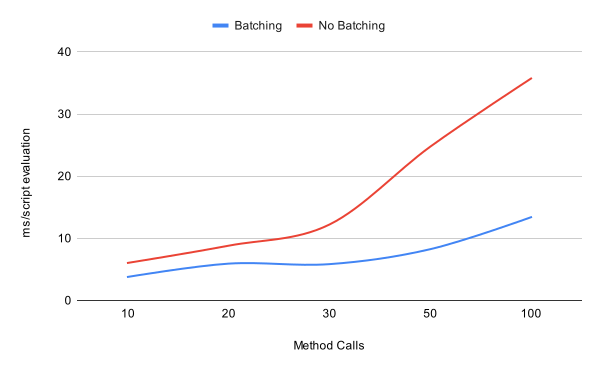
\includegraphics{assets/batching-chart-100-calls.pdf}
    \cprotect\caption{Graph showing the average number of milliseconds taken to run the sttp script shown \hyperref[sec:batching-performance]{above} when \verb|METHOD_CALL_NO| is set to 10, 20, 30, 50, and 100, after running the script 30 times for each \verb|METHOD_CALL_NO|.}
\end{figure}

The graph above shows that when executing up to 20 HTTP method calls within a batch statement, there is a smaller performance increase over executing outside a batch statement, than when executing over 20 HTTP method calls.

\subsubsection{Benchmark 2 - Up to 200 method calls in a batch, 5 iterations each}
\label{sec:batching-benchmark-2}

\begin{center}
    Command that was used to run benchmarks:\\[0.5em]
    \verb|go test -run=XXX -bench="Benchmark(No)?Batch" -benchtime=5x -cpu=8 -count=3|
\end{center}

\begin{figure}[H]
    \centering
    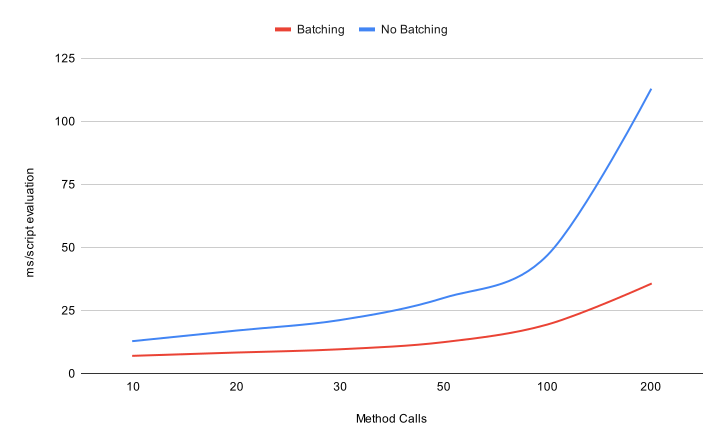
\includegraphics[scale=0.75]{assets/batching-chart-200-calls.pdf}
    \cprotect\caption{Graph showing the average number of milliseconds taken to run the sttp script shown \hyperref[sec:batching-performance]{above} when \verb|METHOD_CALL_NO| is set to 10, 20, 30, 50, 100, and 200, after running the script $5 * 3$ times for each \verb|METHOD_CALL_NO|.}
\end{figure}

The graph above shows a similar result to that of the \hyperref[sec:batching-benchmark-1]{previous benchmark}, but also shows that the growth rate of the milliseconds that it takes to run the test script is a lot less severe when using batching then when not using it at all.

\subsection{Caveats}

\subsubsection{Be sensible.}

A \verb|batch| block will offer no performance boosts if the block contains long running code with sparse usage of HTTP method calls, and could very well be \textbf{detrimental} to the performance of your code. Some general tips...

\begin{itemize}
    \item \textbf{Don't surround long running for or while loops in a batch statement.}
    \item \textbf{Keep expressions and statements without HTTP method calls down to a minimum.}
    \item \textbf{If you are only making a few HTTP method calls rather than 10s or 100s then it might be more performant to remove the batch block.}
    \item \textbf{Do `cache' bulk method calls in a global variable so they are usable throughout the program rather than making many synchronous calls.}
\end{itemize}

It is also worth noting that if there is a \verb|batch| block containing \textbf{zero HTTP method calls}, then the interpreter will \textbf{silently skip the second pass}. There is no need to batch what cannot be batched.

\subsubsection{You cannot batch what has already been batched}

You cannot use a \verb|batch| block within a \verb|batch| block. This inner batch block will throw a \verb|BatchWithinBatch| error. This error is found within Batch AST nodes by checking whether there is a result queue to dequeue from. If there is, then the interpreter knows that this batch block is within another batch block.

\subsubsection{Try-catch surrounding batch blocks}

If an exception occurs in the first or second pass and there is a try-catch surrounding the batch block, then the batch block will be canceled from that point onwards.

If the exception occurs in the thread execution phase then the exception is thrown after all requests are made, in the second pass, in the MethodCall AST node which produced the error.

\cprotect\section{Test suites and the \verb|test| statement}

When running the interpreter from the command line, you can execute entire directory structures of sttp source code. All \verb|test| statements within these source code files will be tested and reported back to the user. A possible use case for this would be testing flows and nested actions within a web API. For instance, take the following directory structure:

\begin{verbatim}
test-web-api/
    user/
        create.sttp
        delete.sttp
        login.sttp
    article/
        create.sttp
        delete.sttp
        retrieve.sttp
        list.sttp
    comment/
        create.sttp
        delete.sttp
        list.sttp
\end{verbatim}

The top level directory encompasses all action sets of the API. For instance, the request \verb|POST /user/login| might be tested with the \verb|test-web-api/user/login.sttp| sttp code. Within this source code file the user could test whether the response from the server is correct, whether the user has been logged in, error cases, etc.

\cprotect\subsection{\verb|test| statement}

The VM keeps an array of the results to all the evaluated test statements in the source code. To evaluate a test, you use the \verb|test| statement. The expression following a \verb|test| statement is evaluated and cast to a Boolean. If the value is \verb|true| then the test has passed, otherwise the test has failed. The result of this test, plus a pointer back to the test statement in the AST, is added to the array of test results within the VM.

A test statement AST node can lie anywhere within a Block AST node, and there can be as many test statements as the user wants within the entire source code. The expression after a test statement \textbf{must exist}, otherwise a parse error will occur.

If a test statement is evaluated within a script that is not executed as a part of a TestSuite, a `temporary' set of TestResults will be created for the duration of the script. This will be used to store the result of any subsequent test statement, so that an error need not be thrown.

\subsection{Execution}

When executing a test suite, the directory structure will be walked in no particular order. Each time a new directory occurs within the current directory, new suite will be created, with the config parameters used to create the current suite, and linked back up to its parent test suite. Each time an sttp source code file is found (\verb|*.sttp|), a new VM is created with the stdout, stderr, and debug file handlers passed to the test suite.

\cprotect\subsubsection{\verb|BreakOnFailure|}

If the \verb|BreakOnFailure| flag is set on the test suite, then the execution of the test suite will exit if any sttp script has a test that fails. Within this failed sttp script, all test statements not yet evaluated by the interpreter, will not be executed whatsoever. Internally, this is achieved by the failed test statement throwing an uncatchable error.

\subsection{Output}
\label{sec:test-suites-and-the-test-statement-test-suite-output}

Once a test suite has been executed, an output will be written to stdout similar to the following:

\begin{verbatim}
PENTHOUSE SUITE: test-web-api  (PASS)
    SUB SUITE: test-web-api/user  (PASS)
        test-web-api/user/create.sttp:2:1 - "test a.code == 201" (PASS)
        test-web-api/user/delete.sttp:2:1 - "test a.code == 200" (PASS)
        test-web-api/user/login.sttp:2:1 - "test a.code == 200" (PASS)
    SUB SUITE: test-web-api/article  (PASS)
        test-web-api/article/create.sttp:2:1 - "test a.code == 201" (PASS)
        test-web-api/article/delete.sttp:2:1 - "test a.code == 200" (PASS)
        test-web-api/article/retrieve.sttp:2:1 - "test a.code == 200" (PASS)
        test-web-api/article/list.sttp:2:1 - "test a.code == 200" (PASS)
    SUB SUITE: test-web-api/comment  (PASS)
        test-web-api/comment/create.sttp:2:1 - "test a.code == 201" (PASS)
        test-web-api/comment/delete.sttp:2:1 - "test a.code == 200" (PASS)
        test-web-api/comment/list.sttp:2:1 - "test a.code == 200" (PASS)
\end{verbatim}

Each directory is treated as a test suite, all inner suites and test statements within the source code is indented. Each line ends with either \verb|(PASS)| or \verb|(FAIL)| indicating whether or not the suite/test statement has passed or failed. If all the test statements within all the source code files and test suites within a suite have passed then that suite will be marked as passing. However, if there is at least one failure, then it will be marked as failing.

\section{External libraries}

\begin{enumerate}
    \item The \href{https://github.com/alecthomas/participle}{participle parser generator} by Alec Thomas. Used for parser and AST generation.
    \item \href{https://pkg.go.dev/github.com/andygello555/gotils}{gotils}: a set of utility functions for Go by Jakab Zeller. Mostly used for some helpful string interpolation functions.
    \item The \href{https://github.com/go-resty/resty}{resty} HTTP/REST client for Go. Used for HTTP Method Calls within sttp.
    \item \href{https://pkg.go.dev/golang.org/x/net}{golang.org/x/net}. Used for its HTML5 compliant parser.
\end{enumerate}

% \begin{center}
%     \begin{verbatim}
%         chunk ::= block
%         block ::= {stat} [retstat]
%         stat ::=  ‘;’ | 
%              varlist ‘=’ explist | 
%              functioncall | 
%              label | 
%              break | 
%              goto Name | 
%              do block end | 
%              while exp do block end | 
%              repeat block until exp | 
%              if exp then block {elseif exp then block} [else block] end | 
%              for Name ‘=’ exp ‘,’ exp [‘,’ exp] do block end | 
%              for namelist in explist do block end | 
%              function funcname funcbody | 
%              local function Name funcbody | 
%              local attnamelist [‘=’ explist] 
%         attnamelist ::=  Name attrib {‘,’ Name attrib}
%         attrib ::= [‘<’ Name ‘>’]
%         retstat ::= return [explist] [‘;’]
%         label ::= ‘::’ Name ‘::’
%         funcname ::= Name {‘.’ Name} [‘:’ Name]
%         varlist ::= var {‘,’ var}
%         var ::=  Name | prefixexp ‘[’ exp ‘]’ | prefixexp ‘.’ Name 
%         namelist ::= Name {‘,’ Name}
%         explist ::= exp {‘,’ exp}
%         exp ::=  nil | false | true | Numeral | LiteralString | ‘...’ |
%              functiondef | prefixexp | tableconstructor | exp binop exp |
%              unop exp 
%         prefixexp ::= var | functioncall | ‘(’ exp ‘)’
%         functioncall ::=  prefixexp args | prefixexp ‘:’ Name args 
%         args ::=  ‘(’ [explist] ‘)’ | tableconstructor | LiteralString 
%         functiondef ::= function funcbody
%         funcbody ::= ‘(’ [parlist] ‘)’ block end
%         parlist ::= namelist [‘,’ ‘...’] | ‘...’
%         tableconstructor ::= ‘{’ [fieldlist] ‘}’
%         fieldlist ::= field {fieldsep field} [fieldsep]
%         field ::= ‘[’ exp ‘]’ ‘=’ exp | Name ‘=’ exp | exp
%         fieldsep ::= ‘,’ | ‘;’
%         binop ::=  ‘+’ | ‘-’ | ‘*’ | ‘/’ | ‘//’ | ‘^’ | ‘%’ | 
%              ‘&’ | ‘~’ | ‘|’ | ‘>>’ | ‘<<’ | ‘..’ | 
%              ‘<’ | ‘<=’ | ‘>’ | ‘>=’ | ‘==’ | ‘~=’ | 
%              and | or
%         unop ::= ‘-’ | not | ‘#’ | ‘~’
%     \end{verbatim}
% \end{center}

% Program  -> Block.
% Block    -> Stmt | Stmt RetStmt.
% Stmts    -> Stmt Stmt |.
% Stmt     -> semi |
%     JSONPath equal Exp |
%     FuncCall |
%     MethodCall |
%     Break |
%     While Exp Do Block End |
%     For Ident equal Exp semi Exp Do Block End |
%     For Ident equal Exp semi Exp semi Exp Do Block End |
%     For Ident In Exp Do Block End |
%     For Ident comma Ident In Exp Do Block End |
%     Function JSONPath FuncBody |
%     If Exp Then Block Elifs End |
%     If Exp Then Block Elifs Else Block End.
% Elifs    -> Elif Exp Then Block Elifs |.
% JSONPath -> Part Parts.
% Parts    -> dot Part Parts |.
% Part     -> Ident Indices.
% Indices  -> sqrL Exp sqrR Indices|.
% RetStmt  -> Return |
%             Return semi |
%             Return Exp semi |
%             Return Exp.
% FuncCall -> JSONPath Args.
% MethodCall -> Method Args.
% FuncBody -> parenL Params parenR Block End | parenL parenR Block End.
% Params   -> Ident Idents.
% Idents   -> comma Ident Idents |.
% Args     -> parenL ExpList parenR | parenL parenR.
% ExpList  -> Exp Exps.
% Exps     -> comma Exp Exps |.

% Exp      -> Prec5T Precs5.
% Precs5   -> Prec5 Precs5|.
% Prec5    -> Prec5Op Prec5T Prec5.
% Prec5Op  -> union.

% Prec5T   -> Prec4T Precs4.
% Precs4   -> Prec4 Precs4|.
% Prec4    -> Prec4Op Prec4T Prec4.
% Prec4Op  -> and.

% Prec4T   -> Prec3T Precs3.
% Precs3   -> Prec3 Precs3|.
% Prec3    -> Prec3Op Prec3T Prec3.
% Prec3Op  -> eq | ne.

% Prec3T   -> Prec2T Precs2.
% Precs2   -> Prec2 Precs2|.
% Prec2    -> Prec2Op Prec2T Prec2.
% Prec2Op  -> lt | gt | lte | gte.

% Prec2T   -> Prec1T Precs1.
% Precs1   -> Prec1 Precs1|.
% Prec1    -> Prec1Op Prec1T Prec1.
% Prec1Op  -> plus | minus.

% Prec1T   -> Factor Precs0.
% Precs0   -> Prec0 Precs0|.
% Prec0    -> Prec0Op Factor Prec0.
% Prec0Op  -> mult | div.

% Factor   -> Null |
%             False |
%             True |
%             Number |
%             StringLit |
%             JSONPath |
%             JSON |
%             FuncCall | MethodCall |
%             AriExp |
%             parenL Exp parenR.

% JSON     -> Object | Array.
% Object   -> curlyL Members curlyR | curlyL curlyR.
% Members  -> Pair Pairs.
% Pairs    -> comma Pair Pairs |.
% Pair     -> Exp colon Exp.
% Array    -> sqrL ExpList sqrR.
